\documentclass[UTF8]{ctexart}
\usepackage{dirtree}
\usepackage{listings}
\usepackage{graphicx}
\usepackage{subfigure}
\usepackage{float}
\usepackage{subfigure}


\title{深度学习实验一四} 
\author{1190200708 熊峰} 
\date{\today}
\begin{document} 
\maketitle 

\newpage
\tableofcontents
\newpage

\section{环境配置}
\subsection{硬件配置}
CPU : Intel(R) Xeon(R) Silver 4214 \par
GPU : TITAN RTX 24G \par
MEM : 128G RAM  \par
\subsection{软件配置}
OS : Ubuntu 20.04.1 LTS \par
PyTorch : Stable 1.11.0  CUDA 11.3 \par
IDE : PyCharm 2021.3.2 \par


\section{文本分类任务}
本部分主要描述模型的结构以及相关代码的编写。  
\subsection{词嵌入}
本部分使用FastText训练词嵌入的模型,将词嵌入的维度设置为300.\par
FastText认为单词的词法结构会携带有关单词含义的重要信息,而传统的单词嵌入并不会考虑这些信息,传统的单词嵌入会为每个单词训练一个唯一的单词嵌入。这对于形态丰富的语言非常重要,在这种语言中,单个单词可能具有大量的形态形式,每种形态形式很少出现,因此很难训练良好的词嵌入。\par
FastText尝试通过将每个单词视为其子单词的集合来解决此问题。为了简单和独立于语言,将子词视为该词的字符n-gram(n元)。一个单词的向量被简单地认为是其组成特征图的所有向量之和。\par
与原始Word2Vec相比,FastText在语法任务上的表现要好得多,尤其是在训练语料库较小的情况下。\par


\subsection{网络结构}
本部分主要描述所使用的网络结构。\par
\subsubsection{RNN}

\begin{figure}[H]
    \begin{center}
        \includegraphics[width=8cm]{\string"RNN".png}
    \caption{RNN Architecture}
    \label{fig:1}
    \end{center}
    \end{figure}
\par
由于为文本分类任务,使用的RNN的结构为序列到类别的模式。\par

输入的样本$x_{1:T}=(x_{1},...,x_{T})$为一个长度为T的序列,输出类别$y{\in}{\{}0,...,9{\}}$,将样本$x$,按不同时刻输入到循环神经网络中,得到不同时刻的隐藏状态$h_{1},...,h_{T}$,可以将$h_{T}$看作整个序列的最终表示,并输入给分类器$g(\cdot)$进行分类。  

如上图\cite{qiu2020nndl}所示,除了使用最后时刻的状态作为整个序列的表示,也可以使用整个状态的所有状态进行平均,并使用这个平均状态作为整个序列的表示,即$\hat{y}=g(\frac{1}{T}\sum\limits_{t=1}^{T}h_{t})$ 



\subsubsection{GRU}
\begin{figure}[H]
    \begin{center}
        \includegraphics[width=10cm]{\string"GRU".png}
    \caption{GRU Architecture}
    \label{fig:2}
    \end{center}
    \end{figure}
\par

GRU的结构如上图所示,它是一种比LSTM网络更加简单的循环神经网络,引入门控机制来控制信息更新的方式。\par
和LSTM不同,GRU不引入额外的记忆单元,GRU网络引入一个更新门来控制当前状态需要从历史状态中保留多少信息,以及需要从候选状态中接受多少新信息。 \par

\subsubsection{LSTM}
\begin{figure}[H]
    \begin{center}
        \includegraphics[width=10cm]{\string"LSTM".png}
    \caption{LSTM Architecture}
    \label{fig:3}
    \end{center}
    \end{figure}
\par

LSTM的结构如上图所示,其为了解决RNN中梯度消失的问题,引入了门控机制,来控制信息传递的路径.LSTM中三个“门”分别为输入门$i_{t}$、遗忘门$f_{t}$和输出门$o_{t}$。\par

输入门$i_{t}$控制当前时刻的候选状态$\tilde{c}_{t}$有多少信息需要保存。\par
遗忘门$f_{t}$控制上一个时刻的内部状态$c_{t}$需要遗忘多少信息。 \par
输出门$o_{t}$控制当前时刻的内部状态$c_{t}$有多少信息需要输出给外部状态。 \par
通过LSTM循环单元,整个网络可以建立较长举例的时序依赖关系。

\subsubsection{BiLSTM}
双向LSTM的结构与LSTM的结构类似,相较于LSTM的主要改进是加上了反向累积的信息。  \par

\subsection{训练过程}
实验中RNN收敛的最慢,迭代次数超过14000次仍未收敛,GRU、LSTM、BiLSTM收敛速度较快。\par
\subsubsection{RNN训练过程}

\begin{figure}[H]
    \begin{minipage}[t]{0.5\linewidth}
        \centering
        \includegraphics[width=\textwidth]{\string"RNNtrainloss".png}
        \centerline{(a) RNN Train Loss}
    \end{minipage}%
    \begin{minipage}[t]{0.5\linewidth}
        \centering
        \includegraphics[width=\textwidth]{\string"RNNtrainF1".png}
        \centerline{(b) RNN Train Micro F1 Score}
    \end{minipage}
    \label{fig:4}
    \caption{RNN Train}
\end{figure}



\subsubsection{GRU训练过程}

\begin{figure}[H]
    \begin{minipage}[t]{0.5\linewidth}
        \centering
        \includegraphics[width=\textwidth]{\string"GRUtrainloss".png}
        \centerline{(a) GRU Train Loss}
    \end{minipage}%
    \begin{minipage}[t]{0.5\linewidth}
        \centering
        \includegraphics[width=\textwidth]{\string"GRUtrainF1".png}
        \centerline{(b) GRU Train Micro F1 Score}
    \end{minipage}
    \label{fig:5}
    \caption{GRU Train}
\end{figure}


\subsubsection{LSTM训练过程}
\begin{figure}[H]
    \begin{minipage}[t]{0.5\linewidth}
        \centering
        \includegraphics[width=\textwidth]{\string"LSTMtrainloss".png}
        \centerline{(a) LSTM Train Loss}
    \end{minipage}%
    \begin{minipage}[t]{0.5\linewidth}
        \centering
        \includegraphics[width=\textwidth]{\string"LSTMtrainF1".png}
        \centerline{(b) LSTM Train Micro F1 Score}
    \end{minipage}
    \label{fig:6}
    \caption{LSTM Train}
\end{figure}

\subsubsection{BiLSTM训练过程}
\begin{figure}[H]
    \begin{minipage}[t]{0.5\linewidth}
        \centering
        \includegraphics[width=\textwidth]{\string"BiLSTMtrainloss".png}
        \centerline{(a) BiLSTM Train Loss}
    \end{minipage}%
    \begin{minipage}[t]{0.5\linewidth}
        \centering
        \includegraphics[width=\textwidth]{\string"BiLSTMtrainF1".png}
        \centerline{(b) BiLSTM Train Micro F1 Score}
    \end{minipage}
    \label{fig:7}
    \caption{BiLSTM Train}
\end{figure}


\subsection{实验结果}
\subsubsection{RNN实验结果}
RNN的实验效果及confusion matrix如下所示:\par

\begin{tabular}{|l|c|c|c|c|} %l(left)居左显示 r(right)居右显示 c居中显示
    \hline 
    class & precision & recall & f1-score & support\\
    \hline 
    Book &0.69&0.76&0.72&770\\
    Pad &0.60&0.67&0.63&2000\\
    Phone &0.00&0.00&0.00&464\\
    Fruit &0.55&0.61&0.58&2000\\
    Shampoo &0.49&0.50&0.49&2000\\
    ElectricWaterHeaters &0.00&0.00&0.00&115\\
    Monmilk &0.52&0.60&0.56&407\\
    Clothe &0.75&0.63&0.69&2000\\
    Computer &0.58&0.76&0.66&798\\
    Hotel &0.92&0.94&0.93&2000\\
    Accuracy& &&0.65&12554\\
    macro avg&0.51&0.55&0.53&12554\\
    weighted avg&0.62&0.65&0.63&12554\\
    \hline 
\end{tabular}

\begin{figure}[H]
    \begin{center}
        \includegraphics[width=9cm]{\string"confusion_Text_RNN".png}
    \caption{RNN confusion matrix}
    \label{fig:8}
    \end{center}
    \end{figure}
\par

\subsubsection{GRU实验结果}
GRU的实验效果及confusion matrix如下所示:\par

\begin{tabular}{|l|c|c|c|c|} %l(left)居左显示 r(right)居右显示 c居中显示
    \hline 
    class & precision & recall & f1-score & support\\
    \hline 
    Book & 0.79 & 0.95 & 0.86 & 770 \\
    Pad & 0.53 & 0.82 & 0.64 & 2000 \\
    Phone &0.00&0.00&0.00&464\\
    Fruit &0.85&0.86&0.85&2000\\
    Shampoo &0.75&0.84&0.79&2000\\
    ElectricWaterHeaters &0.00&0.00&0.00&115\\
    Monmilk &0.00&0.00&0.00&407\\
    Clothe &0.81&0.89&0.85&2000\\
    Computer &0.00&0.00&0.00&798\\
    Hotel &0.93&0.97&0.95&2000\\
    Accuracy & &&0.76&12554\\
    macro avg &0.47 &0.53&0.49&12554\\
    weighted avg & 0.67&0.76&0.70&12554\\
    \hline 
\end{tabular}

\begin{figure}[H]
    \begin{center}
        \includegraphics[width=9cm]{\string"confusion_Text_GRU".png}
    \caption{GRU confusion matrix}
    \label{fig:9}
    \end{center}
    \end{figure}
\par


\subsubsection{LSTM实验结果}
LSTM的实验效果及confusion matrix如下所示:\par

\begin{tabular}{|l|c|c|c|c|} %l(left)居左显示 r(right)居右显示 c居中显示
    \hline 
    class & precision & recall & f1-score & support\\
    \hline 
    Book &0.59 &0.93&0.72&770\\
    Pad &0.56&0.75&0.64&2000\\
    Phone &0.00&0.00&0.00&464\\
    Fruit &0.91&0.84&0.88&2000\\
    Shampoo &0.65&0.86&0.74&2000\\
    ElectricWaterHeaters &0.00&0.00&0.00&115\\ 
    Monmilk &0.00&0.00&0.00&407\\
    Clothe &0.86&0.86&0.86&2000\\
    Computer &0.00&0.00&0.00&798\\
    Hotel &0.90&0.97&0.93&2000\\
    Accuracy & &&0.74&12554\\
    macro avg & 0.45&0.52&0.48&12554\\
    weighted avg &0.65 &0.74&0.69&12554\\
    \hline 
\end{tabular}

\begin{figure}[H]
    \begin{center}
        \includegraphics[width=9cm]{\string"confusion_Text_LSTM".png}
    \caption{LSTM confusion matrix}
    \label{fig:10}
    \end{center}
    \end{figure}
\par

\subsubsection{BiLSTM实验结果}
BiLSTM的实验效果及confusion matrix如下所示:\par

\begin{tabular}{|l|c|c|c|c|} %l(left)居左显示 r(right)居右显示 c居中显示
    \hline 
    class & precision & recall & f1-score & support\\
    \hline 
    Book & 0.94&0.90&0.92&770\\
    Pad &0.78&0.79&0.78&2000\\
    Phone &0.76&0.82&0.79&464\\
    Fruit &0.90&0.90&0.90&2000\\
    Shampoo &0.80&0.83&0.81&2000\\
    ElectricWaterHeaters &0.00&0.00&0.00&115\\
    Monmilk &0.96&0.95&0.96&407\\
    Clothe &0.87&0.88&0.88&2000\\
    Computer &0.84&0.85&0.84&798\\
    Hotel &0.97&0.96&0.97&2000\\
    Accuracy& &&0.87&12554\\
    macro avg & 0.78&0.79&0.79&12554\\
    weighted avg& 0.86&0.87&0.86&12554\\
    \hline 
\end{tabular}

\begin{figure}[H]
    \begin{center}
        \includegraphics[width=9cm]{\string"confusion_Text_BiLSTM".png}
    \caption{BiLSTM confusion matrix}
    \label{fig:11}
    \end{center}
    \end{figure}
\par

\subsubsection{实验结果对比}
本次实验中BiLSTM的效果最好,其相较于LSTM累积了双向的文本的信息,相较于RNN引入了门控机制。LSTM和GRU的效果相似。RNN效果相较于以上模型效果较差一些,此外,RNN收敛的速度也远远慢于上述模型。\par

观察实验效果表,可以看到有些类没有被分出来,一种是比较类似的情况,例如手机、电脑、平板等,可能存在评论类似等情况,一种是样本数量较少时,例如热水器、蒙牛等。\par

在将GRU和LSTM换成BiLSTM后,模型的识别能力大大增强,仅有热水器由于样本量太少,导致模型效果学习不佳。\par



\section{天气预测}

\subsection{数据预处理}
首先对时间的数据进行预处理,直接传入日期会令网络难以学习,进行正余弦处理后使数据之间更加贴近,例如1月12月之间的气候应该使比较接近的,使用正余弦处理可以实现这种效果。 \par
将数据分为训练集和测试集,训练集为2009-2014年的数据集,测试集为2015-2016年的数据集,以七天为时间间隔,对数据进行分割。其中前五天的数据信息为输入的信息,后两天的温度信息作为ground truth。\par 




\subsection{网络结构}
主要使用LSTM网络对天气数据建模,采用异步的时序输入输出方式,采用导师训练过程,输入前五天的信息,使网络预测后两天288个时序点的输出。\par 

\subsection{实验效果}
本次实验记录了网络预测的结果与ground truth的误差,并绘制了相关图片。\par


\begin{figure}[H]
    \centering
    \subfigure[weather 1]{
        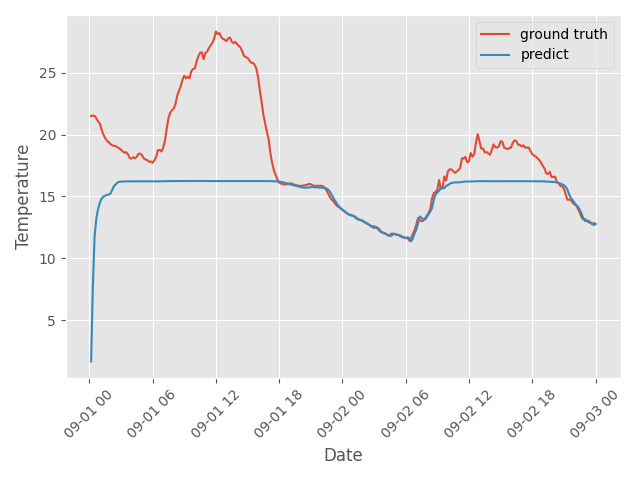
\includegraphics[width=0.3\textwidth]{weather1.png}
    }
    \subfigure[weather 2]{
        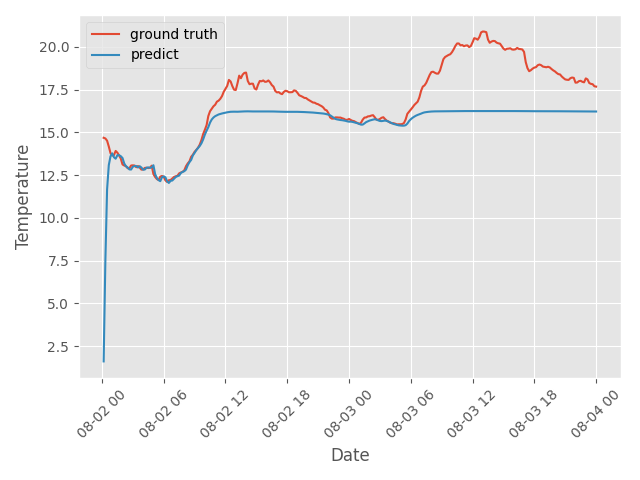
\includegraphics[width=0.3\textwidth]{weather2.png}
    }
    \subfigure[weather 3]{
        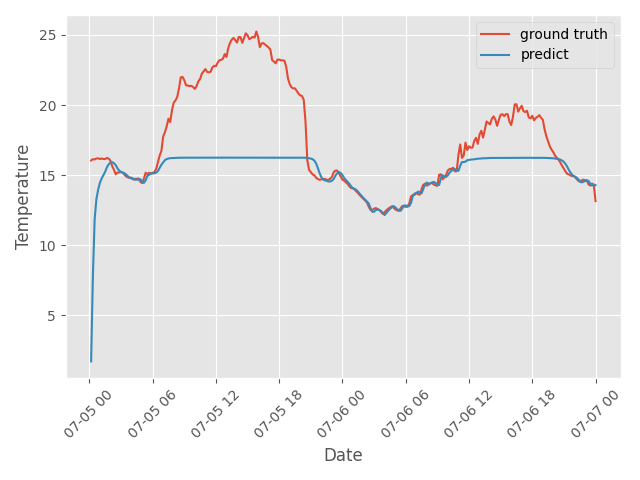
\includegraphics[width=0.3\textwidth]{weather3.png}
    }
    \subfigure[weather 4]{
        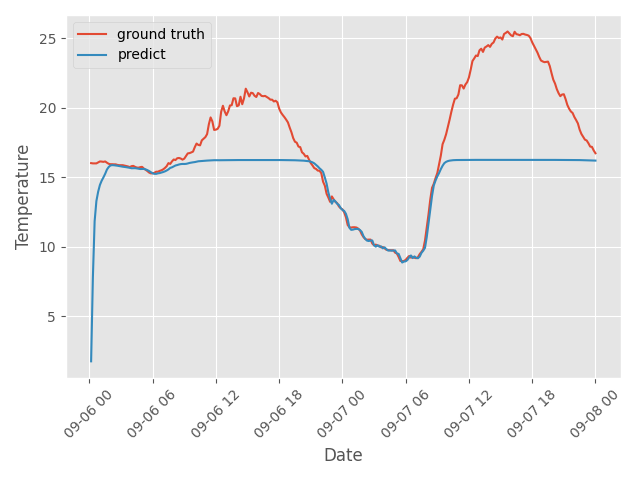
\includegraphics[width=0.3\textwidth]{weather4.png}
    }
    \subfigure[weather 5]{
        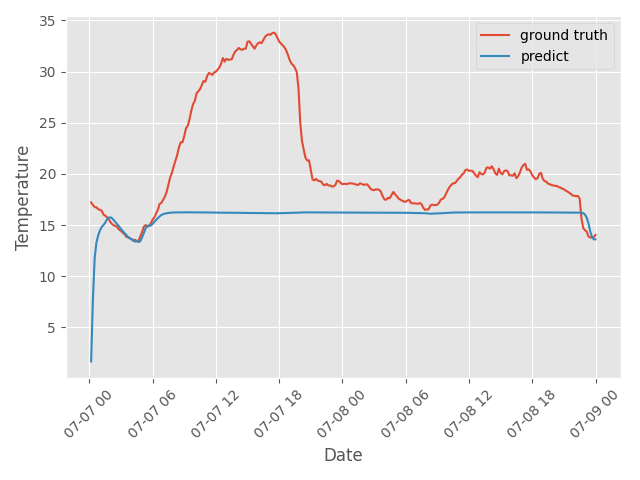
\includegraphics[width=0.3\textwidth]{weather5.png}
    }
    \subfigure[weather 6]{
        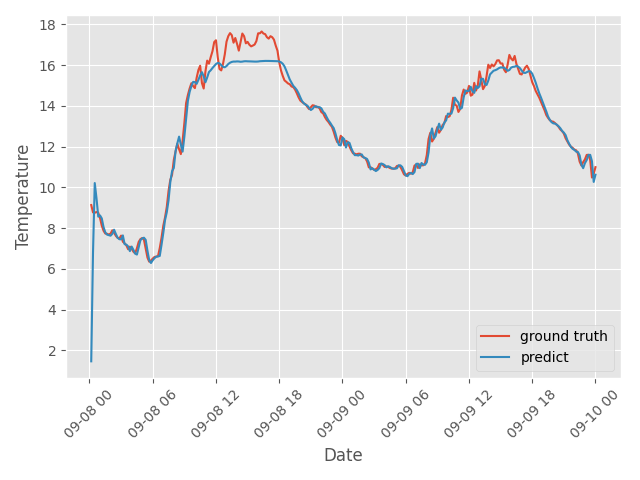
\includegraphics[width=0.3\textwidth]{weather6.png}
    }
    \subfigure[weather 7]{
        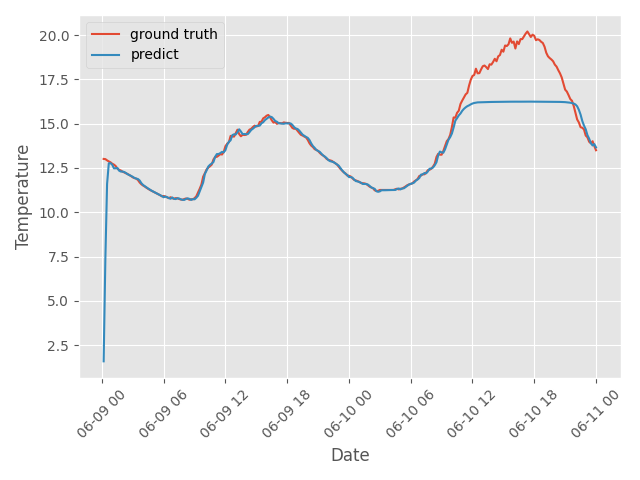
\includegraphics[width=0.3\textwidth]{weather7.png}
    }
    \subfigure[weather 8]{
        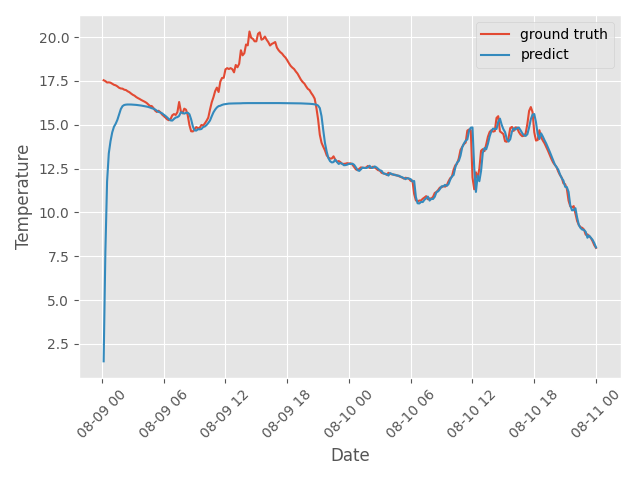
\includegraphics[width=0.3\textwidth]{weather8.png}
    }
    \subfigure[weather 9]{
        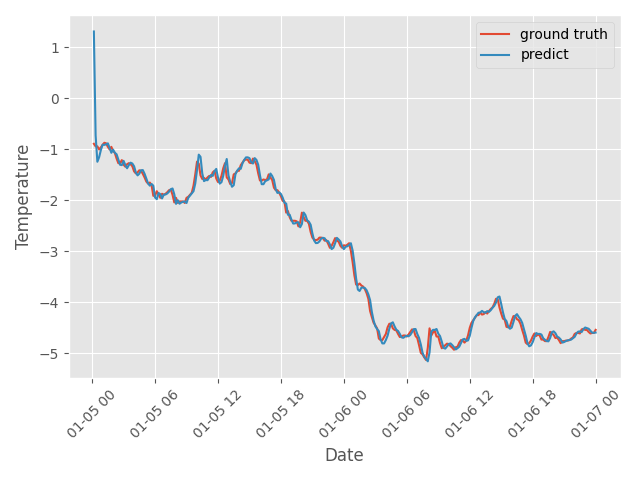
\includegraphics[width=0.3\textwidth]{weather9.png}
    }
    \caption{Temperature Predict}
    \label{fig:12}
\end{figure}

预测的平均绝对误差、绝对误差中位数、平均平方误差、平方误差中位数以及R2Score如下图所示,对于某些样本拟合效果较差:

\begin{figure}[H]
    \begin{center}
        \includegraphics[width=10cm]{\string"error".png}
    \caption{Weather Predict Error}
    \label{fig:13}
    \end{center}
    \end{figure}
\par


\bibliographystyle{unsrt} 
\bibliography{refs}


\end{document}






